Laravel Forge jest narzędziem do wdrażania i konfigurowania aplikacji internetowych. Został opracowany przez twórców szkieletu Laravela, ale może być użyty do zautomatyzowania wdrożenia dowolnej aplikacji internetowej, która korzysta z serwera PHP.

Tworzenie w pełni funkcjonalnego serwera WWW zazwyczaj wymaga instalacji wielu komponentów, takich jak NGINX, MySQL i PHP. Laravel Forge automatyzuje wszystkie niezbędne kroki instalacji i konfiguracji, co pozwala na szybkie uruchomienie witryny.

Po utworzeniu serwera, wdrażanie aktualizacji staje przejrzyste i bezbolesne. Ponadto, można łatwo zarządzać konfiguracją swojej strony internetowej za pomocą interfejsu WWW. Wreszcie, Forge automatycznie udostępnia zaawansowane funkcje bezpieczeństwa, takie jak darmowe certyfikaty SSL (poprzez Let's Encrypt) i automatyczną konfigurację firewalla.

\begin{figure}[!ht]
    \centering
    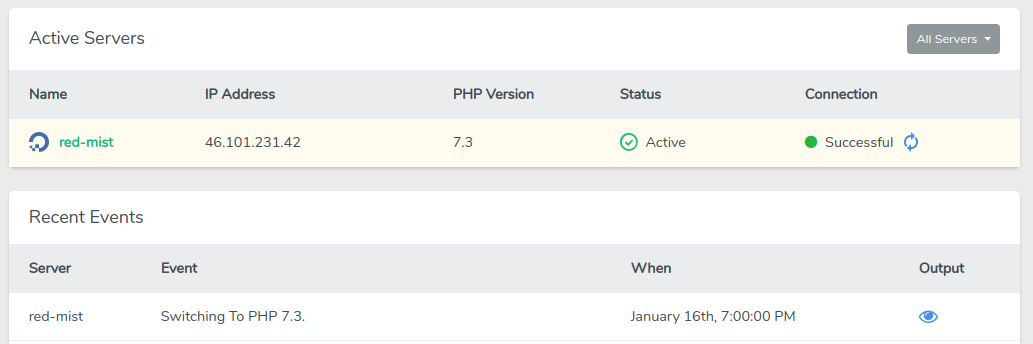
\includegraphics[width=6in]{images/forge.png}
    \caption{Przykład dodania certyfikatu na stronie https://cloud.digitalocean.com \label{fig:forge}}
\end{figure}